\section{Werk}
\hypertarget{RefHeadingToc100333739}{}

\subsection{Werkverzeichnis}
\label{bkm:Ref99364830}\hypertarget{RefHeadingToc100333740}{}\label{bkm:Ref99368924}\subparagraph{Geistliche
Musik}
\begin{flushleft}
\tablefirsthead{}
\tablehead{}
\tabletail{}
\tablelasttail{}
\begin{supertabular}{m{7.6850004cm}m{8.178cm}}
\multicolumn{2}{m{16.063cm}}{{\bfseries Messen}}\\
\textbf{{\textquotedbl}Laurentius{\textquotedbl}-Messe C-Dur op. 14} &
4-st. gem. Chor, Blechbläserquartett, Orgel\\
{\bfseries {\textquotedbl}Mater-Dei{\textquotedbl}-Messe F-Dur op. 16} &
4-st. gem. Chor, Streichquintett, Orgel\\
\textbf{{\textquotedbl}Josephi{\textquotedbl}-Messe F-Dur op. 62} &
4-st. gem. Chor, Soli, 2 Vl., Blechblquat., Orgel\\
\multicolumn{2}{m{16.063cm}}{{\bfseries Tantum ergo}}\\
{\bfseries 4 Tantum ergo op. 32} &
\\
\textbf{ Tantum ergo Nr. 1 Es-Dur op. 11 } &
4-st. gem. Chor, Streichquintett, Orgel\\
\textbf{ Tantum ergo Nr. 2 F-Dur op. 32} &
4-st. gem. Chor, Streichquintett, Orgel\\
\textbf{ Tantum ergo Nr. 3 Es-Dur op. 49} &
4-st. gem. Chor , Streichquintett, Orgel\\
\textbf{ Tantum ergo Nr. 4 A-Dur op. 47} &
4-st. gem. Chor, Streichquintett, Orgel\\
\multicolumn{2}{m{16.063cm}}{{\bfseries Pange lingua}}\\
\textbf{Pange lingua G-Dur }(deutsch) &
4-st. gem. Chor, Blechbläserquartett\\
{\bfseries Pange lingua F-Dur op. 43 } &
4-st. gem. Chor, Orgel\\
{\bfseries Pange lingua Es-Dur op. 46 } &
4-st. gem. Chor, Orgel\\
{\bfseries Pange lingua Es-Dur op. 51 } &
4-st. gem. Chor, Orgel\\
\multicolumn{2}{m{16.063cm}}{{\bfseries Marienlieder}}\\
{\bfseries Ave Maria F-Dur op. 4} &
Unter- und Oberstimme, Orgel\\
{\bfseries Lieder zum Lobe und Preise Mariens} &
\\
\textbf{ Marienlied Nr. 1 F-Dur op. 13 a } &
4-st. gem. Chor, Orgel\\
\textbf{ Marienlied Nr. 2 e-moll op. 19 } &
Sopran-Solo, 4-st. gem. Chor, Orgel\\
\textbf{ Marienlied Nr. 3 F-Dur op. 22 } &
Sopran-Solo, 4-st. gem. Chor, Orgel\\
\textbf{ Marienlied Nr. 4 G-Dur op. 23 } &
Sopran-Solo, 4-st. gem. Chor, Orgel\\
\textbf{ Marienlied Nr. 5 F-Dur op. 28 } &
4-st. gem. Chor, Orgel\\
\textbf{ Marienlied Nr. 6 F-Dur op. 41 } &
4-st. Frauenchor, Orgel\\
\textbf{ Marienlied Nr. 7 G-Dur op. 45 }(fragmentarisch) &
Sopran-Solo, 4-st. gem. Chor, Orgel\\
\textbf{ Marienlied Nr. 8 G-Dur op. 54} &
Sopran-Solo, 4-st. gem. Chor, Orgel\\
\textbf{ Marienlied Nr. 9 G-Dur op. 34} &
4-st. Männerchor\\
\textbf{ Marienlied Nr. 10 F-Dur op. 56 } &
2 Sopran- und Alt-Solo, 4-st. gem. Chor, Orgel\\
\textbf{ Marienlied Nr. 11 F-Dur op. 59} &
Bariton-Solo, 4-st. gem. Chor, Orgel\\
\textbf{ Marienlied Nr. 12 F-Dur op. 63} &
Sopran- und Alt-Solo, Orgel\\
\textbf{ Marienlied (Nr. 13) C-Dur} &
Sopran-Solo, Klavier o. Harmonium\\
\multicolumn{2}{m{16.063cm}}{{\bfseries Grablieder}}\\
\textbf{Grablied für gefallene Soldaten Es-Dur op. 35} &
4-st. gem. Chor, Blechbläserquartett\\
{\bfseries Grablieder op. 35} &
\\
\textbf{ Grablied Nr. 1 Es-Dur op. 35 } &
4-st. gem. Chor, Blechbläserquartett\\
\textbf{ Grablied Nr. 2 Es-Dur} &
4-st. gem. Chor, Blechbläserquartett\\
\textbf{ Grablied Nr. 3 Es-Dur op. 44} &
4-st. gem. Chor, Blechbläserquartett\\
\textbf{ Grablied Nr. 4 F-Dur op. 20 } &
Sopran-Solo, 4-st. gem. Chor, Orgel\\
\multicolumn{2}{m{16.063cm}}{{\bfseries Offertorien}}\\
{\bfseries Offertorium D-Dur op. 26 } &
4-st. gem. Chor, Orgel\\
{\bfseries Offertorium C-Dur op. 30 } &
4-st. gem. Chor, Orgel\\
{\bfseries Offertorium G-Dur op. 48 } &
4-st. Männerchor, Orgel\\
\multicolumn{2}{m{16.063cm}}{{\bfseries Kommunionlieder}}\\
{\bfseries Kommunionlied Es-Dur op. 12} &
4-st. gem. Chor, Orgel\\
{\bfseries Kommunionlied G-Dur op. 21 a} &
4-st. gem. Chor, Orgel\\
{\bfseries Kommunionlied G-Dur op. 21 b} &
4-st. gem. Chor, Orgel\\
{\bfseries Kommunionlied C-Dur op. 37 b} &
4-st. gem. Chor, Orgel\\
\multicolumn{2}{m{16.063cm}}{{\bfseries Veni creator Spiritius}}\\
{\bfseries Veni creator Spiritus B-Dur} &
4-st. Männerchor\\
{\bfseries 11 Veni creator Spiritus op. 15} &
\\
{\bfseries  Veni creator Spiritus C-Dur Nr. 1} &
4-st. gem. Chor\\
\textbf{ Veni creator Spiritus D-Dur Nr. 2} &
4-st. gem. Chor\\
\textbf{ Veni creator Spiritus Es-Dur Nr. 3} &
4-st. gem. Chor\\
\textbf{ Veni creator Spiritus E-Dur Nr. 4} &
4-st. gem. Chor\\
\textbf{ Veni creator Spiritus F-Dur Nr. 5} &
4-st. gem. Chor\\
\textbf{ Veni creator Spiritus Fis-Dur Nr. 6} &
4-st. gem. Chor\\
\textbf{ Veni creator Spiritus G-Dur Nr. 7} &
4-st. gem. Chor\\
\textbf{ Veni creator Spiritus As-Dur Nr. 8} &
4-st. gem. Chor\\
\textbf{ Veni creator Spiritus A-Dur Nr. 9} &
4-st. gem. Chor\\
{\bfseries  Veni creator Spiritus B-Dur Nr. 10} &
4-st. gem. Chor\\
\textbf{ Veni creator Spiritus H-Dur Nr. 11} &
4-st. gem. Chor\\
\multicolumn{2}{m{16.063cm}}{{\bfseries Adjuva nos}}\\
{\bfseries Adjuva nos Es-Dur op. 8 } &
4-st. gem. Chor, Streichquintett, Orgel\\
{\bfseries 8 Adjuva nos op. 15} &
\\
{\bfseries  Adjuva nos C-Dur Nr. 1} &
4-st. gem. Chor\\
{\bfseries  Adjuva nos D-Dur Nr. 2} &
4-st. gem. Chor\\
\textbf{ Adjuva nos Es-Dur Nr. 3} &
4-st. gem. Chor\\
\textbf{ Adjuva nos E-Dur Nr. 4} &
4-st. gem. Chor\\
\textbf{ Adjuva nos F-Dur Nr. 5} &
4-st. gem. Chor\\
\textbf{ Adjuva nos G-Dur Nr. 6} &
4-st. gem. Chor\\
\textbf{ Adjuva nos A-Dur Nr. 7} &
4-st. gem. Chor\\
\textbf{ Adjuva nos B-Dur Nr. 8} &
4-st. gem. Chor\\
\multicolumn{2}{m{16.063cm}}{{\bfseries verschiedene Genre}}\\
{\bfseries Cäcilienlied E-Dur op. 12 b} &
3-st. Frauenchor, Orgel\\
{\bfseries Libera e-moll op. 50} &
4-st. gem. Chor\\
{\bfseries Benedictus G-Dur op. 50} &
4-st. gem. Chor\\
{\bfseries Fronleichnams-Prozessionsgesänge Es-Dur op. 52} &
4-st. gem. Chor, Blechbläserquartett\\
{\bfseries Ecce sacerdos F-Dur op. 57} &
4-st. gem. Chor, Blechbläserquartett, Orgel\\
{\bfseries Juravit Dominus B-Dur op. 58} &
4-st. gem. Chor, Blechbläserquartett, Orgel\\
{\bfseries {\textquotedbl}Ehre sei Gott{\textquotedbl} C-Dur} &
4-st. gem. Chor\\
\textbf{\textit{Herz-Jesu-Litanei }}\textit{(verloren)} &
\\
\end{supertabular}
\end{flushleft}
\subparagraph{Weltliche Musik}
\begin{flushleft}
\tablefirsthead{}
\tablehead{}
\tabletail{}
\tablelasttail{}
\begin{supertabular}{m{7.6850004cm}m{6.642cm}}
\textbf{Marsch {\textquotedbl}In Treue fest!{\textquotedbl} D-Dur } &
Klavier\\
\textbf{Weihegesang Es-Dur }(fragmentarisch) &
4-st. gem. Chor, Blechbläserquartett\\
\textbf{Lied von Gotteszell G-Dur op. 42 }(Arrangement) &
4-st. Männerchor\\
\end{supertabular}
\end{flushleft}
\clearpage\subparagraph[Arrangements]{Arrangements}
\label{bkm:Ref100328080}\begin{flushleft}
\tablefirsthead{}
\tablehead{}
\tabletail{}
\tablelasttail{}
\begin{supertabular}{m{2.848cm}m{7.743cm}m{5.072cm}}
\multicolumn{3}{m{16.063cm}}{{\bfseries Messen}}\\
Schubert, F.  &
{\bfseries Deutsche Messe Es-Dur} &
für 4-st. gem. Chor arrangiert\\
Siebzehnriegel, F. X.  &
{\bfseries Messe zu Ehren der liebreichen Mutter Es-Dur op. 4} &
Bläserquartett hinzugefügt\\
Stein, J.  &
{\bfseries Instrumental-Messe Nr. 6 Es-Dur op. 78} &
Bläserquartett hinzugefügt\\
\multicolumn{3}{m{16.063cm}}{{\bfseries Requiem}}\\
Deschermeier, J.  &
{\bfseries Missa de Requiem Es-Dur op. 90} &
Bläserquartett hinzugefügt\\
Ett, C.  &
{\bfseries Missa pro defunctis Es-Dur} &
Bläserquartett hinzugefügt\\
Gloger, J.  &
{\bfseries Requiem (Missa IV) d-moll op. 27} &
Bläserquartett hinzugefügt\\
Gruber, J.  &
{\bfseries Missa pro defunctis Es-Dur op. 80} &
Bläserquartett hinzugefügt\\
Gruber, J.  &
{\bfseries Requiem in c-moll op. 114} &
Bläserquartett hinzugefügt\\
Huber, H.  &
{\bfseries Requiem mit Libera c-moll op. 21} &
Bläserquartett hinzugefügt\\
Mitterer, I.  &
{\bfseries Missa pro defunctis As-Dur} &
Bläserquartett hinzugefügt\\
\multicolumn{3}{m{16.063cm}}{{\bfseries Tantum ergo}}\\
Bruckner, A.  &
{\bfseries 6 Tantum ergo As-Dur} &
Violinstimmen hinzugefügt\\
\multicolumn{3}{m{16.063cm}}{{\bfseries Pange lingua}}\\
Goller, V.  &
{\bfseries 12 Pange lingua B-Dur op. 5} &
Bläserquartett hinzugefügt\\
\multicolumn{3}{m{16.063cm}}{{\bfseries Marienlieder}}\\
Griesbacher, P.  &
{\bfseries Marienlied {\textquotedbl}O Himmelskönigin{\textquotedbl}
F-Dur op. 137} &
für Solo und 4-st. gem. Chor arrangiert\\
Griesbacher, P.  &
\textbf{Marienlied {\textquotedbl}Wenn mein Schifflein sich will
wenden{\textquotedbl} C-Dur op. 137} &
für Solo und 4-st. gem. Chor arrangiert\\
Hämel, A.  &
\textbf{Marienlied {\textquotedbl}Ein Bildnis ist mir ins Herz
gegraben{\textquotedbl} F-Dur op. 88} &
für 4-st. gem. Chor arrangiert\\
Schächtl, G.  &
{\bfseries Marienlied {\textquotedbl}Maria, lilienreine!{\textquotedbl}
As-Dur op. 2} &
für 4-st. gem. Chor arrangiert\\
\multicolumn{3}{m{16.063cm}}{{\bfseries Trauungslieder}}\\
Lützel, H.  &
{\bfseries Trauungslied {\textquotedbl}Wo du hingehst{\textquotedbl}
Es-Dur} &
für 4-st. gem. Chor arrangiert\\
Silcher, F.  &
\textbf{Trauungslied {\textquotedbl}So nimm denn meine
Hände{\textquotedbl} D-Dur} &
für 4-st. gem. Chor arrangiert\\
\multicolumn{3}{m{16.063cm}}{{\bfseries Grablieder}}\\
Abt, F. W.  &
{\bfseries Grablied {\textquotedbl}Über den Sternen{\textquotedbl} F-Dur
op. 374 Nr. 3} &
für 4-st. gem. Chor arrangiert\\
Braun, A.  &
{\bfseries Grablied Nr. 7 {\textquotedbl}Geht nun hin und grabt mein
Grab{\textquotedbl} B-Dur } &
für 4-st. gem. Chor arrangiert\\
Claudius, G. K.  &
{\bfseries Grablied Nr. 6 {\textquotedbl}Im Grabe ist Ruh{\textquotedbl}
G-Dur } &
für 4-st. gem. Chor arrangiert\\
Donderer, O.  &
{\bfseries Grablied am Grabe eines Helden Es-Dur op. 1} &
Bläserquartett hinzugefügt\\
Engelhart, F. X.  &
\textbf{Trauerlied {\textquotedbl}Friedhofsglocken rufen
klagend{\textquotedbl} Es-Dur op. 77} &
Bläserquartett hinzugefügt\\
Güttler, J.  &
{\bfseries Grablied Nr. 1 {\textquotedbl}Wie war so mild{\textquotedbl}
Es-Dur} &
Bläserquartett hinzugefügt\\
Güttler, J.  &
{\bfseries Grablied Nr. 2 F-Dur} &
Bläserquartett hinzugefügt\\
Güttler, J.  &
\textbf{Grablied Nr. 3 {\textquotedbl}Das liebe treue
Mutterherz{\textquotedbl} Es-Dur} &
Bläserquartett hinzugefügt\\
Haunschild, F.  &
\textbf{Grablied {\textquotedbl}Treues Herz, nun ruh in
Frieden{\textquotedbl} F-Dur} &
Bläserquartett hinzugefügt\\
Kindsmüller, K.  &
{\bfseries Trauerlied für gefallene Helden F-Dur op. 70} &
Bläserquartett hinzugefügt\\
Pleyer, E.  &
{\bfseries Grablied B-Dur op. 50 Nr. 5} &
Bläserquartett hinzugefügt\\
Schröder, F.  &
\textbf{Zum Gedächtnis unserer gefallenen Krieger Es-Dur} &
Bläserquartett hinzugefügt\\
Seitz, F.  &
\textbf{3 Grabgesänge für gef. Krieger F-Dur op. 28} &
Bläserquartett hinzugefügt\\
Tresch, J. B.  &
{\bfseries Am Grabe eines Kriegers Es-Dur} &
für 4-st. gem. Chor arrangiert, Bläserquartett hinzugefügt\\
\multicolumn{3}{m{16.063cm}}{{\bfseries Offertorien}}\\
Goller, V.  &
{\bfseries Offertorium {\textquotedbl}Terra tremuit{\textquotedbl} B-Dur
op. 22 Nr. 23} &
Bläserquartett hinzugefügt\\
Goller, V.  &
{\bfseries Offertorium {\textquotedbl}Tui sunt coeli{\textquotedbl}
C-Dur op. 21 Nr. 8} &
Bläserquartett hinzugefügt\\
Mitterer, I.  &
{\bfseries Festoffertorien C-Dur op. 89} &
Streichquintett hinzugefügt\\
\multicolumn{3}{m{16.063cm}}{{\bfseries Oster-Liturgie}}\\
Schächtl, G.  &
{\bfseries Deutscher Auferstehungs-Chor Es-Dur op. 24} &
Bläserquartett hinzugefügt\\
\multicolumn{3}{m{16.063cm}}{{\bfseries Herz-Jesu-Lieder}}\\
Griesbacher, P.  &
\textbf{Herz-Jesu-Lied {\textquotedbl}O hätt ich tausend
Herzen{\textquotedbl} D-Dur op. 33 Nr. 2} &
für 4-st. gem. Chor arrangiert\\
Griesbacher, P.  &
\textbf{Herz-Jesu-Lied {\textquotedbl}Dem Herzen Jesu
singe{\textquotedbl} C-Dur op. 33 Nr. 1} &
für 4-st. gem. Chor arrangiert\\
Zangl, J. G.  &
\textbf{Herz-Jesu-Lied {\textquotedbl}Ein Herz hab ich
gefunden{\textquotedbl} G-Dur op. 41 Nr. 1} &
Orgelstimme hinzugefügt\\
Zangl, J. G.  &
{\bfseries Herz-Jesu-Lied {\textquotedbl}O Jesus meine Liebe, zieh
gnädig meinen Sinn{\textquotedbl} As-Dur op. 41 Nr. 2}

 &
Orgelstimme hinzugefügt\\
\end{supertabular}
\end{flushleft}
\begin{center}
\tablefirsthead{}
\tablehead{}
\tabletail{}
\tablelasttail{}
\begin{supertabular}{m{9.701cm}}

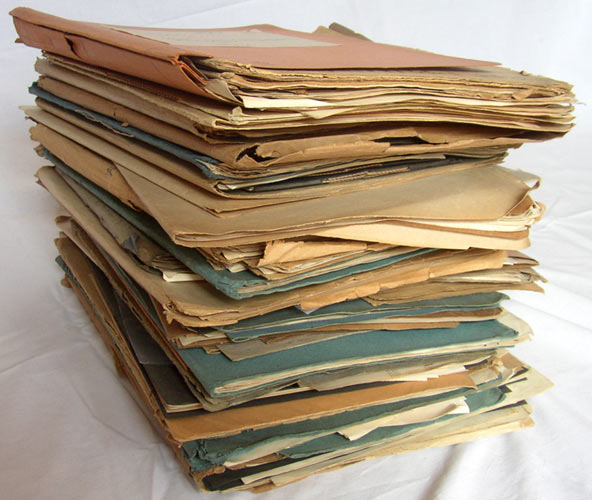
\includegraphics[width=9.491cm,height=8.017cm]{pictures/zulassungsarbeit-img059.jpg}

Abb. \stepcounter{Abb}{\theAbb}: Alle Autographen der Kompositionen von
Högn\\
\end{supertabular}
\end{center}
\clearpage\subparagraph{Anmerkungen zu den Opuszahlen}
Nur als chaotisch kann der Eindruck beschrieben werden, den die
Opuszahlen von Högns Werk auf den Leser machen. Eigentlich sind die
Opuszahlen dafür gedacht, nacheinander im Druck erschienenen Werken
eine fortlaufende Erkennungsnummer zu geben. Da nur der Marsch „In
Treue fest!“ gedruckt wurde, fällt den Nummern bei Högn die Funktion
zu, nacheinander entstandene Werke zu kennzeichnen. Für Verwirrung
sorgen deshalb die vielen doppelten Nummern. So tragen jeweils zwei als
eigenständig anzusehende Werke die Opuszahl 12, 15, 21 und 50. Ebenso
ungewöhnlich erscheint Högns Vorgehensweise, dass er nachträglich
mehrere Werke, die bereits verschiedene Opuszahlen tragen, zu einem
übergeordneten Werkkomplex mit einer neuer Opuszahl zusammenfasste. Die
Komposition „4 Tantum ergo op. 32“ setzt sich etwa aus Stücken mit den
Opusnummern 11, 32, 47 und 49 zusammen. Darüber hinaus passen die 8
Werke ohne Opuszahl nicht recht ins Bild der ansonsten sehr großzügigen
„Opusvergabepraxis.“ Mit dem Lied von Gotteszell G-Dur op. 42 wurde
sogar ein Arrangement gewissermaßen durch die Aufnahme ins Opus
„geadelt“, während hingegen Werke mit weit größerer kompositorischer
Eigenleistung, wie beispielsweise das Grablied Nr. 2 Es-Dur,
unberücksichtig blieben.

\begin{center}
\begin{minipage}{9.241cm}
\begin{center}
\tablefirsthead{}
\tablehead{}
\tabletail{}
\tablelasttail{}
\begin{supertabular}{m{4.5470004cm}m{4.294cm}}

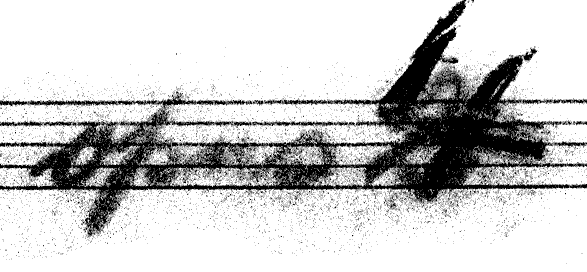
\includegraphics[width=4.364cm,height=2.007cm]{pictures/zulassungsarbeit-img060.png}

Abb. \stepcounter{Abb}{\theAbb}: ausgebesserte Opuszahl auf dem
Autographen des Ave Marias F-Dur op. 4 &

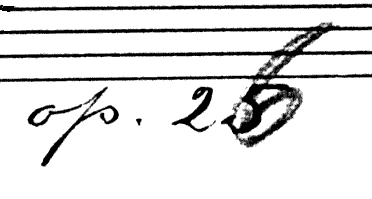
\includegraphics[width=3.739cm,height=2cm]{pictures/zulassungsarbeit-img061.png}

Abb. \stepcounter{Abb}{\theAbb}: ausgebesserte Opuszahl auf dem
Autographen des Offertoriums D-Dur op. 26\\
\end{supertabular}
\end{center}
\end{minipage}
\end{center}
Normalerweise wäre Nummerierung der Werke mit Opuszahlen eine
zuverlässige Informationsquelle bezüglich der Vollständigkeit (siehe
\ref{bkm:Ref98427627} „Zur Frage der Vollständigkeit“, Seite
\pageref{bkm:Ref98427627}) und zeitlichen Entstehung der Kompositionen
(siehe \ref{bkm:Ref98427747} „Entstehungszeit“, Seite
\pageref{bkm:Ref98427747}). Wie können diese Unregelmäßigkeiten erklärt
werden und lassen sich angesichts dieser Unregelmäßigkeiten derartige
Aussagen, wie oben aufgeführt, in Bezug auf Högns Kompositionen machen?

Eine Antwort auf diese Fragen liefert uns die Erörterung der Umstände,
weshalb Högn die offenkundigen Fehler bei der fortlaufenden
Nummerierung unterlaufen sind. Wie man an den Autographen deutlich
erkennen kann, wurden die Opusnummern bis op. 50 nachträglich
hinzugefügt. Högn hatte offensichtlich schon eine Nummerierung seiner
bis dahin geschriebenen Kompositionen in der zeitlichen Abfolge ihrer
Entstehung durchgeführt, als ihm weitere, in der Nummerierung noch
unberücksichtigte Werke unterkamen. Um die Chronologie nicht zu
unterbrechen, entschied er sich, die Opusnummern derjenigen Werke zu
verdoppeln, die nacheinander entstanden waren.

Die Reihenfolge die Opusnummern spiegelt trotz einiger doppelter Nummern
exakt die zeitliche Reihenfolge die Kompositionen wieder. Hätte die
Nummerierung nicht den Sinn gehabt, eine zeitliche Abfolge
herzustellen, sondern die einzelnen Werke besser identifizieren zu
können, wäre es sinnlos gewesen, Nummern zu verdoppeln. Stattdessen
hätte Högn die nächst höhere, noch nicht vergebene Zahl wählen können,
um das noch nicht eingeordnete Werk mit einer eindeutigen
Identifikationsnummer zu belegen. Gruppierungen zu größeren
Werkeinheiten mit neuer Opuszahl, obwohl den untergeordneten Werken
schon Opusnummern vergeben worden sind, stiften zwar etwas Verwirrung,
rütteln aber nicht an der Aussagekraft der untergeordneten Opuszahl,
bezüglich der Entstehungszeit der einzelnen Werke.

Die Existenz der doppelten Nummern, relativiert dagegen die Aussagekraft
der Opuszahlen in Hinblick auf die Frage der Vollständigkeit der Werke
erheblich. Es ist nicht abzusehen, wie viele verschollene Werke mit
gleicher Opuszahl eine Lücke im vorliegenden Werkverzeichnis
geschlossen hätten.

Die Tatsache, dass es doppelte Opuszahlen gibt, kann auch in der
Erklärung, weshalb einige Werke keine Opusnummer tragen,
Richtungweisend sein. Ist es nicht unlogisch, dass Högn einerseits
durch doppelte Opuszahlen „gewaltsam“ versuchte, Werke nachträglich ins
Opus hereinzunehmen und dadurch ein unübersichtliches Bild seines
Gesamtwerks erzeugt, anderseits mancher nicht weniger wertvollen
Komposition eine Opuszahl verwehrt? Viel einleuchtender ist es deshalb,
dass diese Werke mit wenigen Ausnahmen ursprünglich sehr wohl eine
Opuszahl trugen. Wie an den erhaltenen Autographen zu sehen ist, hatte
Högn nur in den seltensten Fällen an alle Bestandteile seines
handgeschriebenen Notenmaterials Opusnummern vermerkt.
Höchstwahrscheinlich sind deshalb bei den Werken ohne Opuszahl nur die
unnummerierten Bestandteile erhalten. Die folgende Tabelle soll bei
jedem einzelnen Werk das Fehlen der Opuszahl begründen und außerdem
eine Vermutung liefern, welche Opuszahl dieses Werk ursprünglich
getragen haben könnte:

\clearpage\begin{flushleft}
\tablefirsthead{}
\tablehead{}
\tabletail{}
\tablelasttail{}
\begin{supertabular}{|m{4.991cm}|m{1.5519999cm}|m{9.12cm}|}
\hline
\textbf{Werk ohne Opusnr.} &
\textbf{Mögl. Opusnr. } &
{\bfseries Begründung für das/die}\\\hline
Marsch {\textquotedbl}In Treue fest!{\textquotedbl} D-Dur  &
1 &
\textbf{Fehlen: }Drucklegung des Marsches vor der Nummerierung

\textbf{Vermutung:} Erstes gedrucktes Werk\\\hline
Grablied Nr. 2 Es-Dur &
36, 38,

39, 40 &
\textbf{Fehlen:} Verlorene Autographen, an denen die Opusnummer vermerkt
war

\textbf{Vermutung:} Fehlende Opuszahlen zwischen Grablied Nr. 1 op. 35
und Grablied Nr. 3 op. 44\\\hline
Herz-Jesu-Litanei &
53, 55,

60, 61 &
\textbf{Fehlen:} Werk ist komplett verschollen

\textbf{Vermutung:} Titel bekannt aus Briefen des Jahres 1948,
wahrscheinlich daher späte Entstehung \\\hline
{\textquotedbl}Ehre sei Gott{\textquotedbl} C-Dur &
53, 55,

60, 61 &
\textbf{Fehlen:} Verlorene Autographen, an denen die Opusnummer vermerkt
war

\textbf{Vermutung:} Deutscher Text, daher Entstehung im Vorfeld des II.
Vatikanischen Konzils, wahrscheinlich deswegen späte Entstehungszeit
\\\hline
Pange lingua (deutsch) G-Dur &
53, 55,

60, 61 &
\textbf{Fehlen:} Verlorene Autographen, an denen die Opusnummer vermerkt
war

\textbf{Vermutung:} Deutscher Text, daher Entstehung im Vorfeld des II.
Vatikanischen Konzils, wahrscheinlich deswegen späte Entstehungszeit ab
45 \\\hline
Marienlied (Nr. 13) C-Dur

 &
64 &
\textbf{Fehlen:} Verlorene Autographen, an denen die Opusnummer vermerkt
war

\textbf{Vermutung:} Letzte erhaltene Komposition\\\hline
Veni creator Spiritus B-Dur &
{}- &
\textbf{Fehlen:} Frühe Version des Veni creator Spiritus D-Dur op. 15
Nr. 2\\\hline
Weihegesang Es-Dur &
{}- &
\textbf{Fehlen:} Verworfen bevor Nummerierung durchgeführt wurde
(NS-Musik)\\\hline
\end{supertabular}
\end{flushleft}